\documentclass[11pt,a4paper,ngerman,openany]{report}
\usepackage[ngerman]{babel}
\usepackage[T1]{fontenc}
\usepackage[utf8]{inputenc}
\usepackage{geometry}
\usepackage{graphicx}
\usepackage{booktabs}
\usepackage{array}
\usepackage{tabularx}
\usepackage{float}
\usepackage{pdfpages}
\usepackage{enumitem}
\usepackage[hidelinks]{hyperref}

\geometry{left=2.5cm,right=2.5cm,top=2.5cm,bottom=2.5cm}
\setlength{\parindent}{0pt}
\setlength{\parskip}{0.2em}

\begin{document}
\hypersetup{pageanchor=false}

% =========================
% 1) TITELSEITE (1 Seite)
% =========================
\begin{titlepage}
    \centering
    \vspace*{0.5cm}

    
\includegraphics[width=0.58\textwidth]{../Summary_Felix_N/figures/JLU_Giessen-Logo.png}\\[1.8cm]

    {\Large Gruppennummer: 308}\\[0.3cm]
    \rule{\linewidth}{0.2mm}\\[0.2cm]
    {\huge\bfseries Neuronales Netz f\"ur den kalifornischen Hauspreis-Datensatz}\\
    \rule{\linewidth}{0.2mm}\\[1.6cm]

    \begin{minipage}{0.52\textwidth}
        \begin{flushleft}
            \textbf{\large Portfolio von:}\\[0.3em]
            Florian Adamczyk\\
            Matrikelnummer: 8105234\\[1.0em]

            \textbf{Rolle in der Gruppe:}\\
            Gruppenmitglied (nicht Sprecher)
        \end{flushleft}
    \end{minipage}
    \begin{minipage}{0.44\textwidth}
        \begin{flushleft}
            \textbf{\large \"Ubrige Gruppenmitglieder:}\\[0.3em]
            Bj\"orn Becker\\
            Felix Hollfoth\\
            Felix Neumann\\
            Kolja Scriba\\[1.0em]

            \textbf{Sprecherin der Gruppe:}\\
            Felix Neumann
        \end{flushleft}
    \end{minipage}\\[1.8cm]

    \begin{minipage}{0.88\textwidth}
        \begin{center}
            Modul: K\"unstliche Intelligenz I\\
            Dozenten: Prof. Dr. Christian Heiliger, Dr. Jan-Matthis Waack\\
            Semester: Wintersemester 2025/26\\
            Abgabetermin: 15.04.2026
        \end{center}
    \end{minipage}

    \vfill
\end{titlepage}

\clearpage
\hypersetup{pageanchor=true}
\pagenumbering{arabic}
\setcounter{page}{1}

% =========================
% 2) ZUSAMMENFASSUNG DES LOGBUCHS (genau 4 Seiten)
% =========================
\section{Zusammenfassung des Logbuchs}
\label{sec:zusammenfassung}

\subsection*{2.1 Fragestellung, Ziel und eigener Arbeitsanteil}
Die zentrale Aufgabenstellung war, f\"ur den California-Housing-Datensatz ein neuronales Netz zu entwickeln und dessen Leistung gegen eine lineare Regression einzuordnen [W1], [W2].

Meine pers\"onliche Leitfrage war: \textit{Wie kann ich die Projektbasis so aufbauen, dass alle Teammitglieder reproduzierbar auf denselben Daten und Metriken arbeiten, und wie weit l\"asst sich dadurch die NN-Performance im Vergleich zur Baseline verbessern?}

Ich war nicht Sprecher der Gruppe, habe aber in der Fr\"uhphase die technische Grundlage gelegt: Repository-Struktur, Abh\"angigkeitsmanagement, gemeinsame Python-Hilfsmodule, Notebook-Templates und Support f\"ur Git/VS-Code im Team.

Die zusammengefassten Aussagen dieses Kapitels sind auf die Logbucheintr\"age im \hyperref[sec:logbuch-anhang]{Anhang} zur\"uckf\"uhrbar. Die Orientierung dazu steht in \hyperref[tab:logbuch-navigator]{Tabelle~\ref*{tab:logbuch-navigator}}.

\begin{table}[H]
\centering
\caption{Logbuch-Navigator (klickbarer Bezug zum Anhang)}
\label{tab:logbuch-navigator}
\begin{tabular}{p{1.5cm}p{2.3cm}p{8.2cm}}
\toprule
Eintrag & Datum & Schwerpunkt \\
\midrule
1 & 11.02.26 & Git-Workflow, nbstripout-Recherche und Einf\"uhrung \\
2 & 17.02.26 & Repository-Struktur, Bereinigung, Team-Onboarding \\
3 & 20.-25.02.26 & Masterplan, Aufgaben\"ubersicht, utils-Module, Notebook-Grundger\"uste \\
4 & 23.-26.02.26 & Neuronale Netze (Modelle 1-5), Vergleich zur Baseline \\
5 & 14.-26.03.26 & Team-Support in Git/VS-Code, finale Notebook-L\"aufe, Portfoliostart \\
\bottomrule
\end{tabular}
\end{table}

\vfill
\begin{flushright}
\textit{Zusammenfassung Seite 1 von 4}
\end{flushright}
\newpage

\subsection*{2.2 Vorarbeit: Infrastruktur als Grundlage der Gruppenleistung}
Die Vorarbeit war auf Reproduzierbarkeit ausgerichtet: einheitliche Umgebungen (README + requirements.txt), sauberes Git-Handling mit nbstripout [W4] und gemeinsame Auswertestandards.

\textbf{Vollst\"andige Methodenliste der von mir geschriebenen utils-Funktionen}

\small
\begin{tabularx}{\textwidth}{>{\raggedright\arraybackslash}p{3.8cm}X}
\toprule
\textbf{Funktion} & \textbf{Kurzfunktion} \\
\midrule
\texttt{load\_raw\_data} & Datensatz laden (einheitlicher Startpunkt). \\
\texttt{clean\_data} & Cut-offs/Ausrei\ss{}er entfernen (98\%-Quantil-Regel). \\
\texttt{load\_and\_clean\_data} & Lade- und Bereinigungspfad in einem Schritt. \\
\texttt{get\_train\_test\_split} & Fester 80/20-Split, Seed 42, optionale Skalierung. \\
\texttt{evaluate\_model} & R\textsuperscript{2}/MAE/RMSE f\"ur Train und Test aus Modellobjekt. \\
\texttt{evaluate\_predictions} & R\textsuperscript{2}/MAE/RMSE direkt aus Vorhersagen (z. B. Keras). \\
\texttt{evaluate\_test\_predictions} & Kompakte Testmetriken f\"ur Einzelvergleiche. \\
\texttt{add\_result} & Ergebnis in globale Vergleichsliste eintragen. \\
\texttt{compare\_models} & Vergleichstabelle aller Modelle erzeugen/sortieren. \\
\texttt{reset\_results} & Vergleichsliste zur\"ucksetzen. \\
\texttt{save\_fig} & Einheitlicher PNG/PDF-Export nach results. \\
\texttt{plot\_predicted\_vs\_actual} & Soll-Ist-Plot mit Ideallinie. \\
\texttt{plot\_residuals} & Residuen gegen Vorhersage visualisieren. \\
\texttt{plot\_feature\_importances} & Feature-Wichtigkeiten geordnet darstellen. \\
\texttt{plot\_correlation\_heatmap} & Korrelationsmatrix als Heatmap. \\
\texttt{plot\_histograms} & Verteilungen aller Spalten in einem Raster. \\
\texttt{plot\_features\_vs\_target} & Feature-Ziel-Scatterplots automatisiert erzeugen. \\
\bottomrule
\end{tabularx}
\normalsize

Diese Vorarbeit war f\"ur die Gruppe zentral, weil dadurch alle Modellvergleiche auf derselben Daten- und Metrikbasis stattfinden konnten.

\vfill
\begin{flushright}
\textit{Zusammenfassung Seite 2 von 4}
\end{flushright}
\newpage

\subsection*{2.3 Modellweg vor der Kernaufgabe NN}
Vor dem eigentlichen NN-Training habe ich mehrere methodische Stufen aufgebaut bzw. vorbereitet und dokumentiert:

\begin{itemize}[leftmargin=*,itemsep=0.2em,topsep=0.2em]
    \item \textbf{EDA} (Notebook 0a): Datenverst\"andnis, Cut-off-Erkennung, Ausrei\ss{}er-Analyse, Korrelationen.
    \item \textbf{Baseline lineare Regression} (Notebook 0b): Referenzwert f\"ur alle weiteren Modelle.
    \item \textbf{LASSO/Ridge} (Notebook 01): Regularisierung, Skalierungseffekte, polynomiale Erweiterungen.
    \item \textbf{Ensemble} (Notebook 03): Random Forest und Gradient Boosting f\"ur starke nichtlineare Benchmarks.
    \item \textbf{kNN} (Notebook 04): distanzbasiertes Modell, deutlicher Skalierungsbedarf.
\end{itemize}

Die Baseline aus der linearen Regression liegt bei etwa $R^2_{Test}=0.6326$ und markiert damit den Minimalstandard f\"ur den NN-Vergleich. Genau dieser Vergleich ist in der Aufgabenstellung explizit gefordert [W1].

\begin{figure}[H]
    \centering
    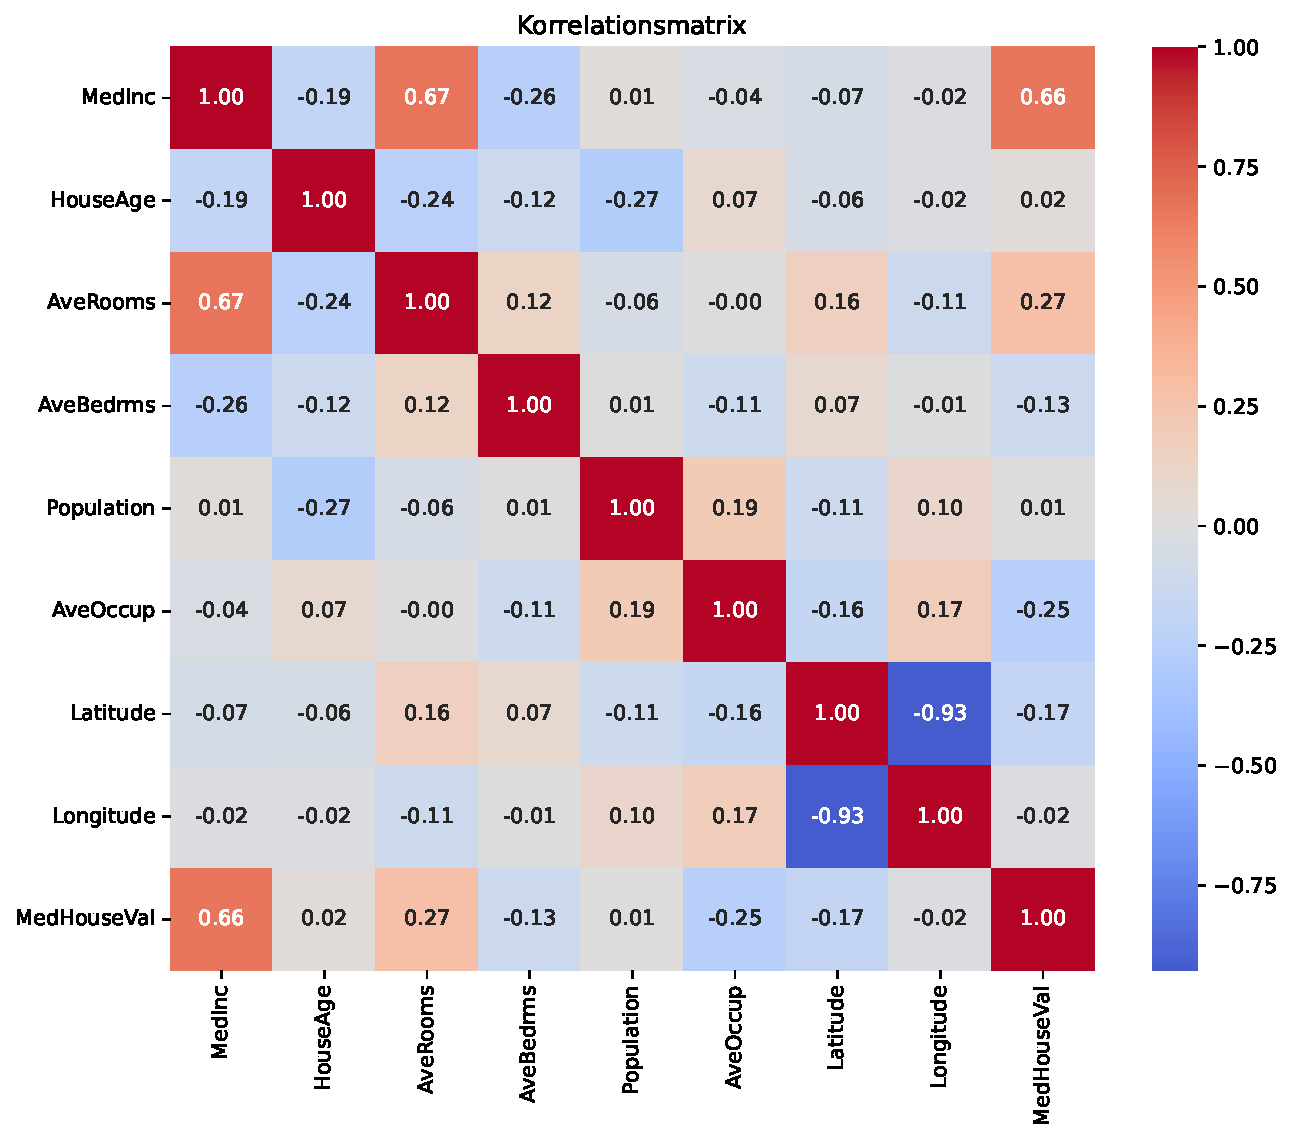
\includegraphics[width=0.47\textwidth]{figures/eda_correlation_heatmap.pdf}
    \hfill
    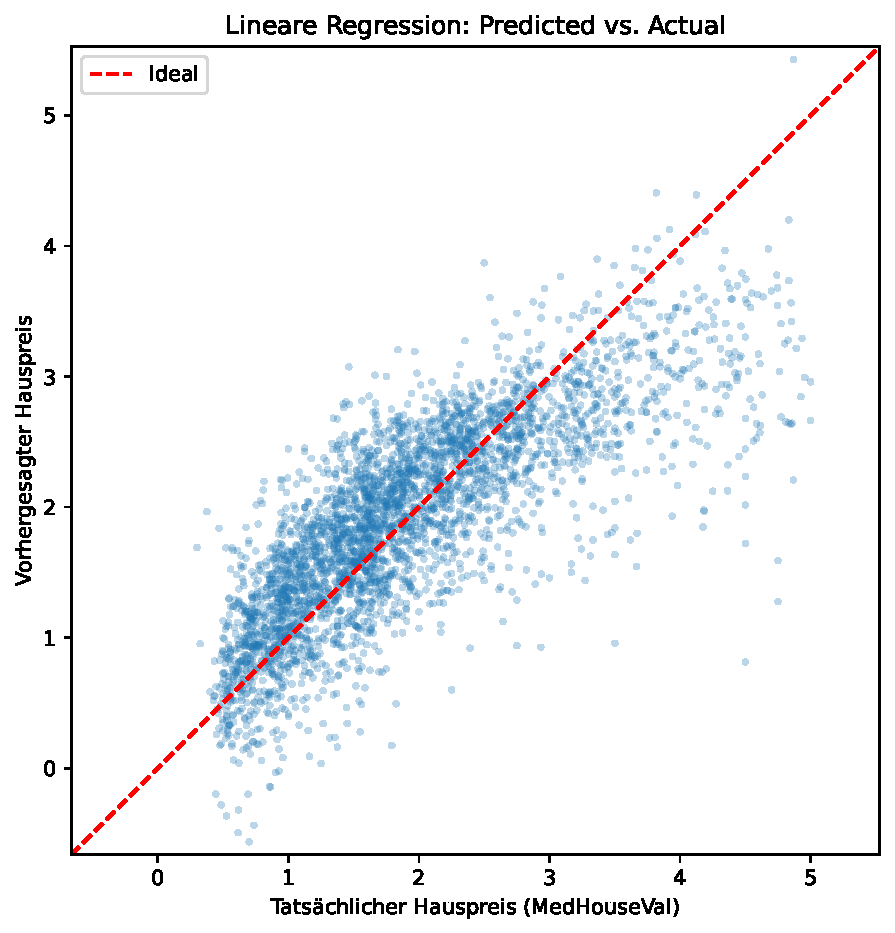
\includegraphics[width=0.47\textwidth]{figures/baseline_pred_vs_actual.pdf}
    \caption{Links: EDA-Korrelationsmatrix. Rechts: Baseline (lineare Regression) mit sichtbaren systematischen Abweichungen.}
    \label{fig:eda-baseline}
\end{figure}

Inhaltlich entstand so ein methodischer Pfad vom Datenverst\"andnis \"uber klassische Regressionsverfahren bis zum neuronalen Netz.

\vfill
\begin{flushright}
\textit{Zusammenfassung Seite 3 von 4}
\end{flushright}
\newpage

\subsection*{2.4 Kernaufgabe: Neuronales Netz, Ergebnisse, Grenzen, Zwischenstand}
Im Notebook \texttt{05\_Neural\_Network\_Florian.ipynb} habe ich mehrere Architekturen schrittweise getestet (von einem kleinen Netz bis zu einem tieferen Modell mit Dropout). Die Eingaben wurden standardskaliert, trainiert wurde mit Adam und MSE als Loss [W3], [W5].

\textbf{Kernresultat:} Das beste von mir trainierte Modell (Architektur [128, 64, 32, 16] mit Dropout) erreicht auf dem Testset einen klar besseren Wert als die lineare Baseline.

\begin{table}[H]
\centering
\caption{Direkter Vergleich Baseline vs. bestes NN-Modell}
\label{tab:nn-vs-lr}
\begin{tabular}{lccc}
\toprule
Modell & $R^2$ Test & MAE Test & RMSE Test \\
\midrule
Lineare Regression & 0.6326 & 0.4341 & 0.5778 \\
Bestes NN (Florian) & 0.7795 & 0.3066 & 0.4480 \\
\bottomrule
\end{tabular}
\end{table}

\begin{figure}[H]
    \centering
    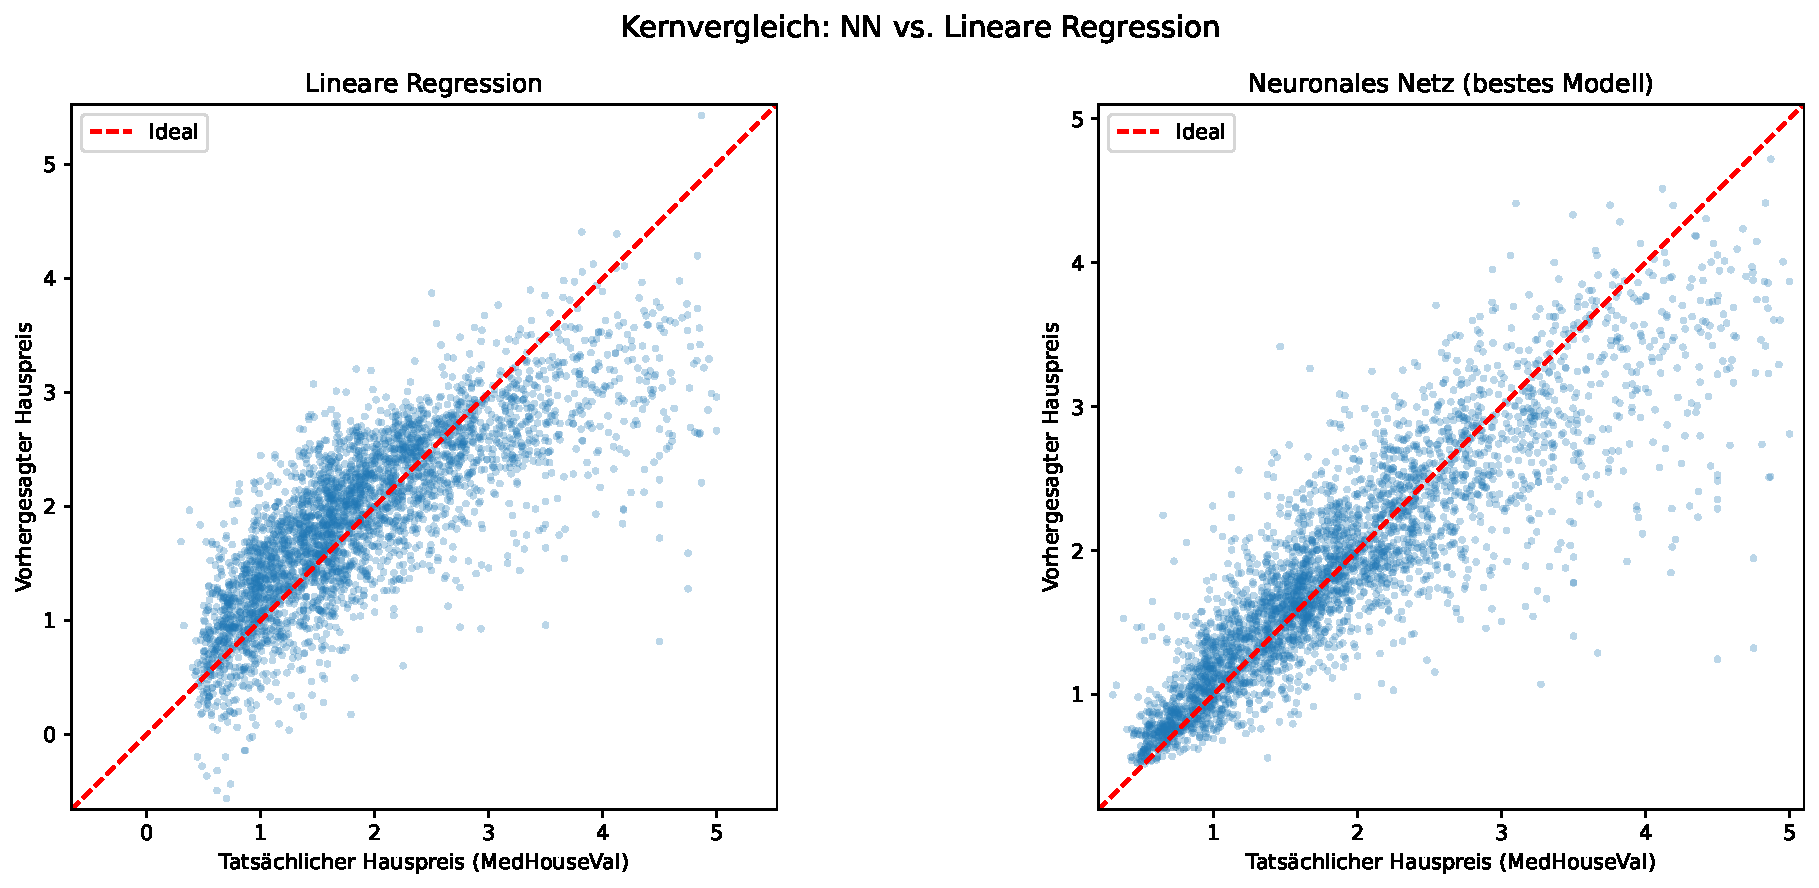
\includegraphics[width=0.66\textwidth]{figures/nn_vs_linear_regression.pdf}
    \caption{Kernvergleich aus dem Projekt: lineare Regression gegen bestes NN-Modell.}
    \label{fig:nn-vs-lr}
\end{figure}

\textbf{Schwierigkeiten und Grenzen}
\begin{itemize}[leftmargin=*,itemsep=0.15em,topsep=0.15em]
    \item TensorFlow-/Python-Kompatibilit\"at im Team (insbesondere unterschiedliche Betriebssysteme) [W3].
    \item Erh\"ohter Abstimmungsaufwand durch unterschiedliche Git-Erfahrung in der Gruppe.
    \item Methodische Grenze: Das NN ist leistungsstark, aber deutlich schlechter interpretierbar als lineare Modelle.
\end{itemize}

\textbf{Erreichter Zwischenstand}
\begin{itemize}[leftmargin=*,itemsep=0.15em,topsep=0.15em]
    \item Reproduzierbare Projektinfrastruktur steht und wurde im Team genutzt.
    \item Baseline und klassische Modelle sind dokumentiert und als Vergleich verf\"ugbar.
    \item Ein belastbarer NN-Verbesserungsschritt gegen\"uber der Baseline wurde nachgewiesen.
\end{itemize}

Damit liegt ein begr\"undeter, methodisch nachvollziehbarer Zwischenstand vor, kein behauptetes Endoptimum. Die Detailnachweise stehen im \hyperref[sec:logbuch-anhang]{Logbuch-Anhang}.

\vfill
\begin{flushright}
\textit{Zusammenfassung Seite 4 von 4}
\end{flushright}

\newpage

% =========================
% 3) EINSCHÄTZUNG DER GRUPPENMITGLIEDER (1 Seite)
% =========================
\section{Einsch\"atzung der Gruppenmitglieder}

Die folgenden Formulierungen sind als konkrete Platzhalter angelegt und werden vor Abgabe final personalisiert.

\small
\begin{tabularx}{\textwidth}{>{\raggedright\arraybackslash}p{3.2cm}X}
\toprule
\textbf{Mitglied} & \textbf{St\"arke / Schw\"ache (arbeitsbezogen)} \\
\midrule
Bj\"orn Becker & St\"arke: sehr strukturierte Ergebnisaufbereitung. Schw\"ache (final konkretisieren): in der Fr\"uhphase zeitlich begrenzte Verf\"ugbarkeit. \\
Felix Hollfoth & St\"arke: sauberes Hyperparameter-Testing. Schw\"ache (final konkretisieren): Einzelschritte mussten sp\"ater st\"arker integriert werden. \\
Felix Neumann (Sprecherin) & St\"arke: klare Koordination in der Schlussphase. Schw\"ache (final konkretisieren): bei parallelen Arbeitspaketen erh\"ohter Abstimmungsaufwand. \\
Kolja Scriba & St\"arke: belastbare Beitr\"age zu Modellvarianten. Schw\"ache (final konkretisieren): Mehraufwand durch unterschiedliche Entwicklungsumgebungen. \\
Florian Adamczyk (Selbst) & St\"arke: fr\"uhe Infrastrukturarbeit als Team-Beschleuniger. Schw\"ache (final konkretisieren): weniger Zeit f\"ur eigenes Feintuning durch Support-Aufgaben. \\
\bottomrule
\end{tabularx}
\normalsize

\newpage

% =========================
% 4) QUELLEN UND HILFSMITTEL (1 Seite)
% =========================
\section{Quellen und Hilfsmittel}

\small
\subsection*{4.1 Webseiten (mit Zugriffsdatum)}
\begin{itemize}[leftmargin=*,itemsep=0.05em,topsep=0.05em]
    \item [W1] Aufgabenblatt Projekt KI I, Gruppe 308 (Stud.IP, Version vom 03.02.2026), Zugriff: 10.04.2026.
    \item [W2] \href{https://scikit-learn.org/stable/modules/generated/sklearn.datasets.fetch_california_housing.html}{Scikit-learn: California Housing Dataset}, Zugriff: 10.04.2026.
    \item [W3] \href{https://www.tensorflow.org/install/pip}{TensorFlow Installation / Kompatibilit\"at}, Zugriff: 10.04.2026.
    \item [W4] \href{https://github.com/kynan/nbstripout}{nbstripout (GitHub)}, Zugriff: 10.04.2026.
    \item [W5] \href{https://scikit-learn.org/stable/modules/model_evaluation.html}{Scikit-learn Metriken (R\textsuperscript{2}, MAE, RMSE)}, Zugriff: 10.04.2026.
\end{itemize}

\subsection*{4.2 B\"ucher und Fachliteratur}
\begin{itemize}[leftmargin=*,itemsep=0.05em,topsep=0.05em]
    \item [L1] Russell, S.; Norvig, P. (2021): \textit{Artificial Intelligence: A Modern Approach}. 4th ed., Pearson.
    \item [L2] Srivastava, N. et al. (2014): Dropout: A Simple Way to Prevent Neural Networks from Overfitting. \textit{Journal of Machine Learning Research}, 15, 1929-1958.
\end{itemize}

\subsection*{4.3 Verwendete Software und Werkzeuge}
Python 3.13 (projektweit prim\"ar), TensorFlow/Keras, scikit-learn, pandas, numpy, matplotlib, Jupyter, VS Code, Git/GitHub, nbstripout.

\subsection*{4.4 Einsatz generativer KI (transparent dokumentiert)}
Als Hilfsmittel f\"ur Strukturierung, sprachliche \"Uberarbeitung und Qualit\"atssicherung wurde ein KI-Assistenzsystem genutzt.
Beispielhafte Prompts:
\begin{itemize}[leftmargin=*,itemsep=0.05em,topsep=0.05em]
    \item \glqq Erstelle eine Gliederung f\"ur ein nicht-sprecher Portfolio mit 7 Seiten Hauptteil.\grqq{}
    \item \glqq Formuliere eine knappe, sachliche Einordnung von Overfitting im NN-Vergleich.\grqq{}
\end{itemize}
\normalsize

\label{lastmainpage}

\newpage

% =========================
% 5) ANHANG: LOGBUCH (nicht im Seitenumfang)
% =========================
\section*{Anhang: Logbuch}
\label{sec:logbuch-anhang}
Das vollst\"andige Logbuch ist als Pflichtanhang beigef\"ugt und dokumentiert die Arbeitsschritte chronologisch.

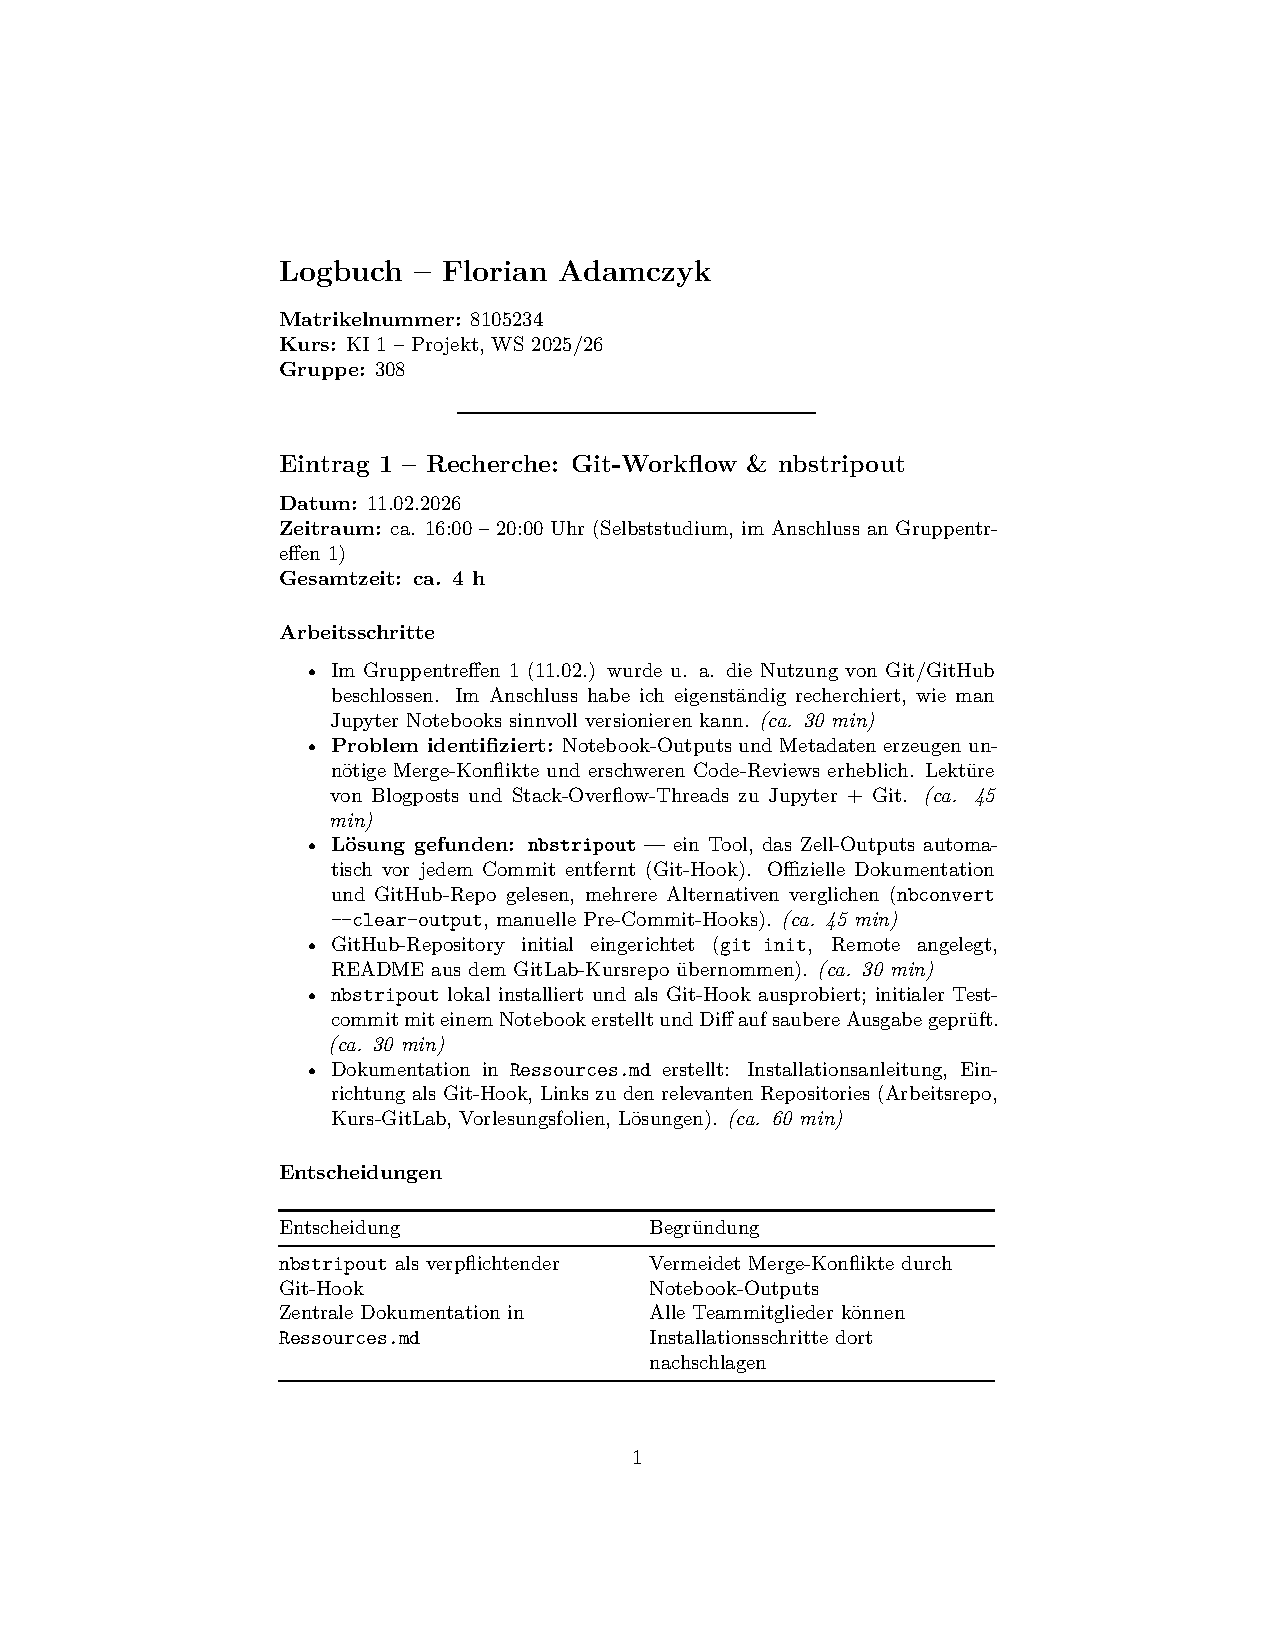
\includepdf[pages=-,pagecommand={\thispagestyle{plain}}]{../Logbuch_Florian_Adamczyk.pdf}

\end{document}
